%%%%%%%%%%%%%%%%%%%%%%%%%%%%%%%%%%%%%%%%%%%%%%%%%%%%%%%%%%%%%%%%%%%%%%%%%%%%%%%%
%2345678901234567890123456789012345678901234567890123456789012345678901234567890
%        1         2         3         4         5         6         7         8

\documentclass[letterpaper, 10 pt, conference]{ieeeconf}  % Comment this line out
                                                          % if you need a4paper
%\documentclass[a4paper, 10pt, conference]{ieeeconf}      % Use this line for a4
                                                          % paper

\IEEEoverridecommandlockouts                              % This command is only
                                                          % needed if you want to
                                                          % use the \thanks command
\overrideIEEEmargins
% See the \addtolength command later in the file to balance the column lengths
% on the last page of the document



% The following packages can be found on http:\\www.ctan.org
%\usepackage{graphics} % for pdf, bitmapped graphics files
%\usepackage{epsfig} % for postscript graphics files
%\usepackage{mathptmx} % assumes new font selection scheme installed
%\usepackage{times} % assumes new font selection scheme installed
%\usepackage{amsmath} % assumes amsmath package installed
%\usepackage{amssymb}  % assumes amsmath package installed

\title{\LARGE \bf
Decentralised Market-Based Strategy for Cooperative Multi-Robot Exploration 
}

%\author{ \parbox{3 in}{\centering autor1*
%         \thanks{*Use the $\backslash$thanks command to put information here}\\
%         Faculty of Electrical Engineering, Mathematics and Computer Science\\
%         University of Twente\\
%         7500 AE Enschede, The Netherlands\\
%         {\tt\small h.kwakernaak@autsubmit.com}}
%         \hspace*{ 0.5 in}
%         \parbox{3 in}{ \centering autor2**
%         \thanks{**The footnote marks may be inserted manually}\\
%        Department of Electrical Engineering \\
%         Wright State University\\
%         Dayton, OH 45435, USA\\
%         {\tt\small pmisra@cs.wright.edu}}
%}
\author{Ana Batinovic, Juraj Orsulic, Stjepan Bogdan
	\thanks{Authors are with the University of Zagreb, Faculty of Electrical Engineering  and Computing, LARICS Laboratory for Robotics and Intelligent Control Systems, Unska 3, 10000 Zagreb, Croatia
        {\tt\small (ana.batinovic, juraj.orsulic, stjepan.bogdan) at fer.hr}}}%

\begin{document}



\maketitle
\thispagestyle{empty}
\pagestyle{empty}


%%%%%%%%%%%%%%%%%%%%%%%%%%%%%%%%%%%%%%%%%%%%%%%%%%%%%%%%%%%%%%%%%%%%%%%%%%%%%%%%
\begin{abstract}

This work presents a novel approach to autonomous decentralised multi-robot frontier exploration and mapping of an unknown area based on the market model. The exploration algorithm enables mobile robots to communicate among each other, to negotiate and to become dispersed throughout the environment. The mobile robot team simultaneously explores the environment, discovers frontier points (points on the border between the explored and unexplored space), and negotiates by fully connected graph and event-based communication. During the negotiation process, the amount of information exchanged between the robots is limited to data about the frontier points. The main goal is to allocate the mobile robots to target frontier points in the environment in a way which minimises the overall exploration time. The proposed strategy has been implemented in a simulation environment and compared with a centralised strategy. The simulation results demonstrate improved behaviour of the decentralised multi-robot strategy in terms of total exploration time and path length. 

\end{abstract}

 
%%%%%%%%%%%%%%%%%%%%%%%%%%%%%%%%%%%%%%%%%%%%%%%%%%%%%%%%%%%%%%%%%%%%%%%%%%%%%%%%
\section{INTRODUCTION}
Analysis and synthesis of decentralised multi-robot systems belong to core robotics problems that have drawn significant attention in last few decades. The coordination of a mobile robot team during the exploration of an unknown area is a common problem encountered in many applications, such as search and rescue \cite{rescue}, cleaning \cite{cleaning1}, \cite{cleaning2}, warehousing \cite{Wurman}, or planetary exploration \cite{planetary}, to name a few. Due to the fact that autonomous multi-robot systems are entering society domain and as such will interact with people on daily basis, development of efficient coordination algorithms becomes inevitable.

 Like in the human world, robots can be more effective when they work together. Moreover, a robot team can accomplish a predefined task much quicker than a single robot can \cite{free-market}. Another advantage of mobile robot teams arises from the possibility of merging overlapping sensor information, which in turn can help to compensate for sensor uncertainty \cite{segmentation}.
If is done properly, multi-robot coordination can lead to i) task accomplishment in the shortest possible time, ii) increased robustness, iii) higher map quality (in case of exploration task), and finally iv) the completion of tasks impossible for a single robot to perform \cite{survey-analysis}.

We consider the problem of an autonomous multi-robot exploration with decentralised coordination strategy based on the market model. The laser scan and odometry sensor measurements of the mobile robot represent input data for a Simultaneous Localisation and Mapping (SLAM) module. In this work, for map building we use a submap-based graph SLAM method -- Google Cartographer \cite{cartographer} -- which, however, in the simulation uses the ground truth mobile robot poses (\textit {perfect localisation}) from the Stage simulator \cite{Stage} in order to eliminate the SLAM algorithm uncertainty. The module also implements frontier detection according to \cite{juraj}. A result of frontier detection are the points on the border of the explored and unexplored space in the environment - \textit{frontier points} shown in the Fig. \ref{fig:environment}. The result of frontier detection is a dense set of frontier points, thus we use a filter to get a more manageable number of the frontier points \cite{Umari}. The decentralised strategy based on the market model module acquires the frontier points from the filter module and assigns mobile robots to target points. Afterwards, the algorithm for path planning and following navigates the mobile robot toward the target point (Fig. \ref{fig:exploration-strategy}).      

\begin{figure}{}
    \centering
	\fbox{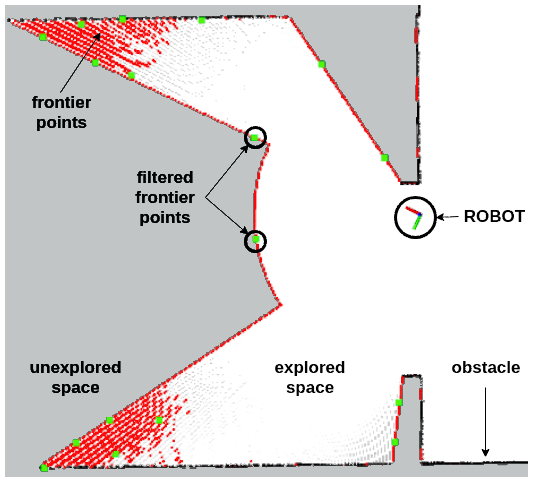
\includegraphics[width=0.85\columnwidth]{frontier_rviz_vol3.png}}
	\caption {The description of the environment. A 2D map is represented with an occupancy grid that divides the map into cells: the white cells describe explored and grey cells unexplored space, while the black cells define obstacles. The frontier detector publishes frontier points (red) and the filter module publishes filtered frontier points (green).}
	\label{fig:environment}
\end{figure}

\begin{figure}
    \centering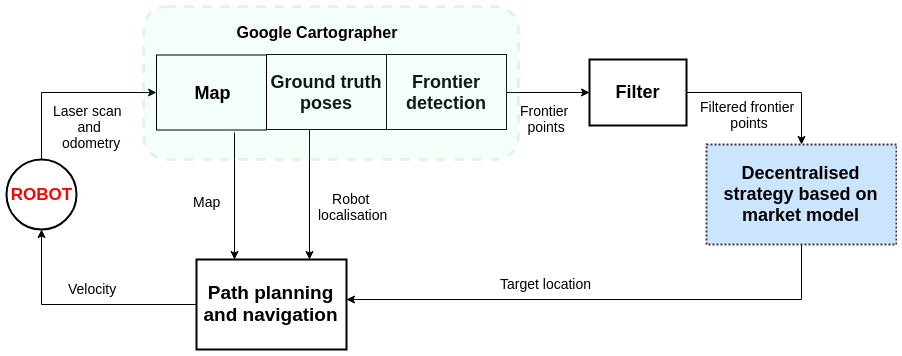
\includegraphics[width=1.0\columnwidth]{diagram_exploration2.png}
	\caption{Overall schematic diagram of the decentralised exploration algorithm in the simulator.}
   \label{fig:exploration-strategy}
\end{figure}

Since the main goal is to achieve faster exploration and better coordination among the mobile robots, our decentralised market-based strategy ensures that the mobile robots become dispersed throughout the environment. Moreover, the mobile robots are dispersed in the environment to accomplish the mission as fast as possible. It is assumed that communication among the mobile robots is modelled by a fully connected graph.

The rest of the paper is organised as follows. The related work is presented in the next section. In Section III the exploration strategy based on market model is described. Simulation results are presented in Section IV, and in the final section a conclusion is given.

\section{RELATED WORK}

Algorithms for assigning robots to target points can be grouped into centralised and decentralised algorithms. 
Centralised task assignment for a multi-robot system may be less practical due to communication limits \cite{free-market}, robustness issues \cite{survey-analysis}, or time required for algorithm execution and scalability \cite{Julia}. In the centralised approach, each mobile robot receives tasks assigned from a single central \emph{leader} using a centralised planning algorithm. During communication between the central leader and the mobile robots, information about the mobile robot poses is shared in order to perform real time mobile robot task allocation. The central leader may be a computer or a robot.

The centralised algorithm described in \cite{burgard} improves robustness, but the negotiation process is complex because the coordination of mobile robots is performed by a central \emph{executive} which creates a global map and executes auction with the  bids from the mobile robots, while in the same time assigning tasks according to the received bids. The auctioneer thus offers a task and other mobile robots compete by bidding. The winner is the robot with the highest revenue (or inversely, with the lowest cost).

In a decentralised approach, the mobile robots are completely autonomous in the exploration process. Each mobile robot has its own local knowledge of the world and can decide its future actions by taking into account its current context and task, its own capacities and the capacities of the other mobile robots, through a negotiation process \cite{Yan}. Moreover, it usually has better reliability, flexibility, adaptability and robustness. 

One of the most representative decentralised approaches is a market model.
The general concept of the market-based approaches includes independence of the mobile robots in terms of planning, and the ability of mobile robots to take team resources into account. It is shown in \cite{usporedba} when different team sizes are included, the decentralised market method has an advantage over the centralised approach in terms of travelled distance.

Authors in \cite{market-economy} use a market architecture for the multi-robot mapping and exploration problem that aims to maximise the difference between the benefit and the cost to achieve the same objective as in the proposed approach (minimise the overall exploration time). However, the proposed approach takes into account an occupancy function which makes mobile robots more dispersed in the environment. Furthermore, we introduce a decentralised market-based strategy that implements event-based communication between mobile robots, reducing the amount of information used in the negotiation process. Similarly to Michael et al. \cite{Michael}, we propose a strategy in which mobile robots are able to take part in negotiation for target point assignment with the assumption that the agents have knowledge of all target points, while we assume that only a single mobile robot can be assigned to a specific target point.  

We have also compared a centralised strategy based on the approach described in \cite{burgard} that also takes into account cost and utility functions proposed in the next section with the proposed decentralised strategy based on market model. The central control agent in the centralised strategy implementation is a computer.

A popular approach for an unknown area exploration is the frontier based exploration algorithm introduced by Yamauchi \cite{Yamauchi}. The idea is to route mobile robots to the frontier. The frontier edges detection can be achieved using RRT (Rapidly Exploring Random Tree) algorithm by Umari and Mukhopadhyay \cite{Umari}. The RRT algorithm is biased towards unexplored regions and provides a general approach which can be extended to higher dimensional spaces. However, RRT algorithm proved not to be fast enough in instances when larger environments were explored, so we opted to use a dense frontier detection method \cite{juraj}.   

\section{APPROACH}

The previous work presented a multi-robot exploration system that can efficiently explore unknown terrain, and is robust to robot failures. Our approach accomplishes the same using a strategy based on the market model. 
In this paper we determine the target points for each mobile robot in the team using an objective function which is a combination of frontier point cost, utility (information gain) and the frontier occupancy function. 

\subsection{Market-based strategy} 

At the core of our approach is negotiation between mobile robots during exploration. The mobile robots exchange information under the assumption of a fully connected graph, where all mobile robots communicate with each other and in the negotiation process each mobile robot takes into account the data received from all other mobile robots.

Every mobile robot $i$ gets the list of frontier points:

\begin{equation}
   \boldsymbol{y}=\begin{bmatrix}
    \boldsymbol{y_{0}} & \boldsymbol{y_{1}} & \boldsymbol{y_{2}} & \hdots & \boldsymbol{y_{M}}
\end{bmatrix},
\end{equation}

where $M$ is  the number of frontier points, and every list member is a vector consisting of the $x$ and $y$ coordinates. 

\begin{equation}
   \boldsymbol{y}=\begin{bmatrix}
   \begin{bmatrix}
           x_{0} \\
           y_{0} 
   \end{bmatrix}
    \begin{bmatrix}
         x_{1} \\
         y_{1} 
    \end{bmatrix}
    \begin{bmatrix}
         x_{2} \\
         y_{2} 
    \end{bmatrix}
    \hdots
    \begin{bmatrix}
         x_{M} \\
         y_{M} 
    \end{bmatrix}
\end{bmatrix}.
\end{equation}


We define the frontier point weight as a function of cost, utility and frontier occupancy. If $i$ is the index of the mobile robot, and $j$ is the index of the frontier point, then the cost function: $C_{ij}$: $R$ \(\rightarrow \text{$\mathbb{R}^{+}$}\) is a mapping from the set of resources $R$ to a positive real number. $C_{ij}$ describes the cost of $i$th robot to visit the $j$th frontier point. The cost can be a function of time, energy or, like in our case, the estimated distance travelled by mobile robot to reach the target frontier point. The estimated distance is approximated using Euclidean distance between the mobile robot position $\boldsymbol{p_{i}}$ and the frontier point position $\boldsymbol{q_{j}}$:

\begin{equation}\small
    C_{ij}=d(\boldsymbol{p_{i}}, \boldsymbol{q_{j}}) = \sqrt{(p_{ix}-q_{jx})^{2}+(p_{iy}-q_{jy})^{2}}.
    \label{cost}
\end{equation}

The utility function $U_{ij}$:  \(\text{$\mathcal {M}$}\) \(\rightarrow \text{$\mathbb{R}^{+}$}\) returns a positive real number from the occupancy grid \(\text{$\mathcal {M}$}\). The cells of \(\text{$\mathcal {M}$}\) may be marked as explored space, unexplored space or obstacle. The utility function is proportional to the number of the unexplored cells ($c$) within a fixed distance from the frontier point $j$ in the previous defined radius $r$: 

\begin{equation}
    U_{ij} = \lambda_{u}c,
\end{equation}

where $\lambda_{u}$ is a constant determined experimentally. When the function $U_{ij}$ is taken into account, the mobile robot will prefer frontier points that are surrounded by more unexplored space even if they are a little bit further. 
It is assumed that the mobile robot will detect all unexplored cells around the assigned frontier point after reaching it. 

\begin{figure*}[h!]
     \begin{center}
     \setcounter{subfigure}{0}
%
        \subfigure[\hspace{0.1cm} Coverage ratio over time in the office scenario for centralised multi-robot exploration.]{%
            \label{fig:office_coverage_c}
            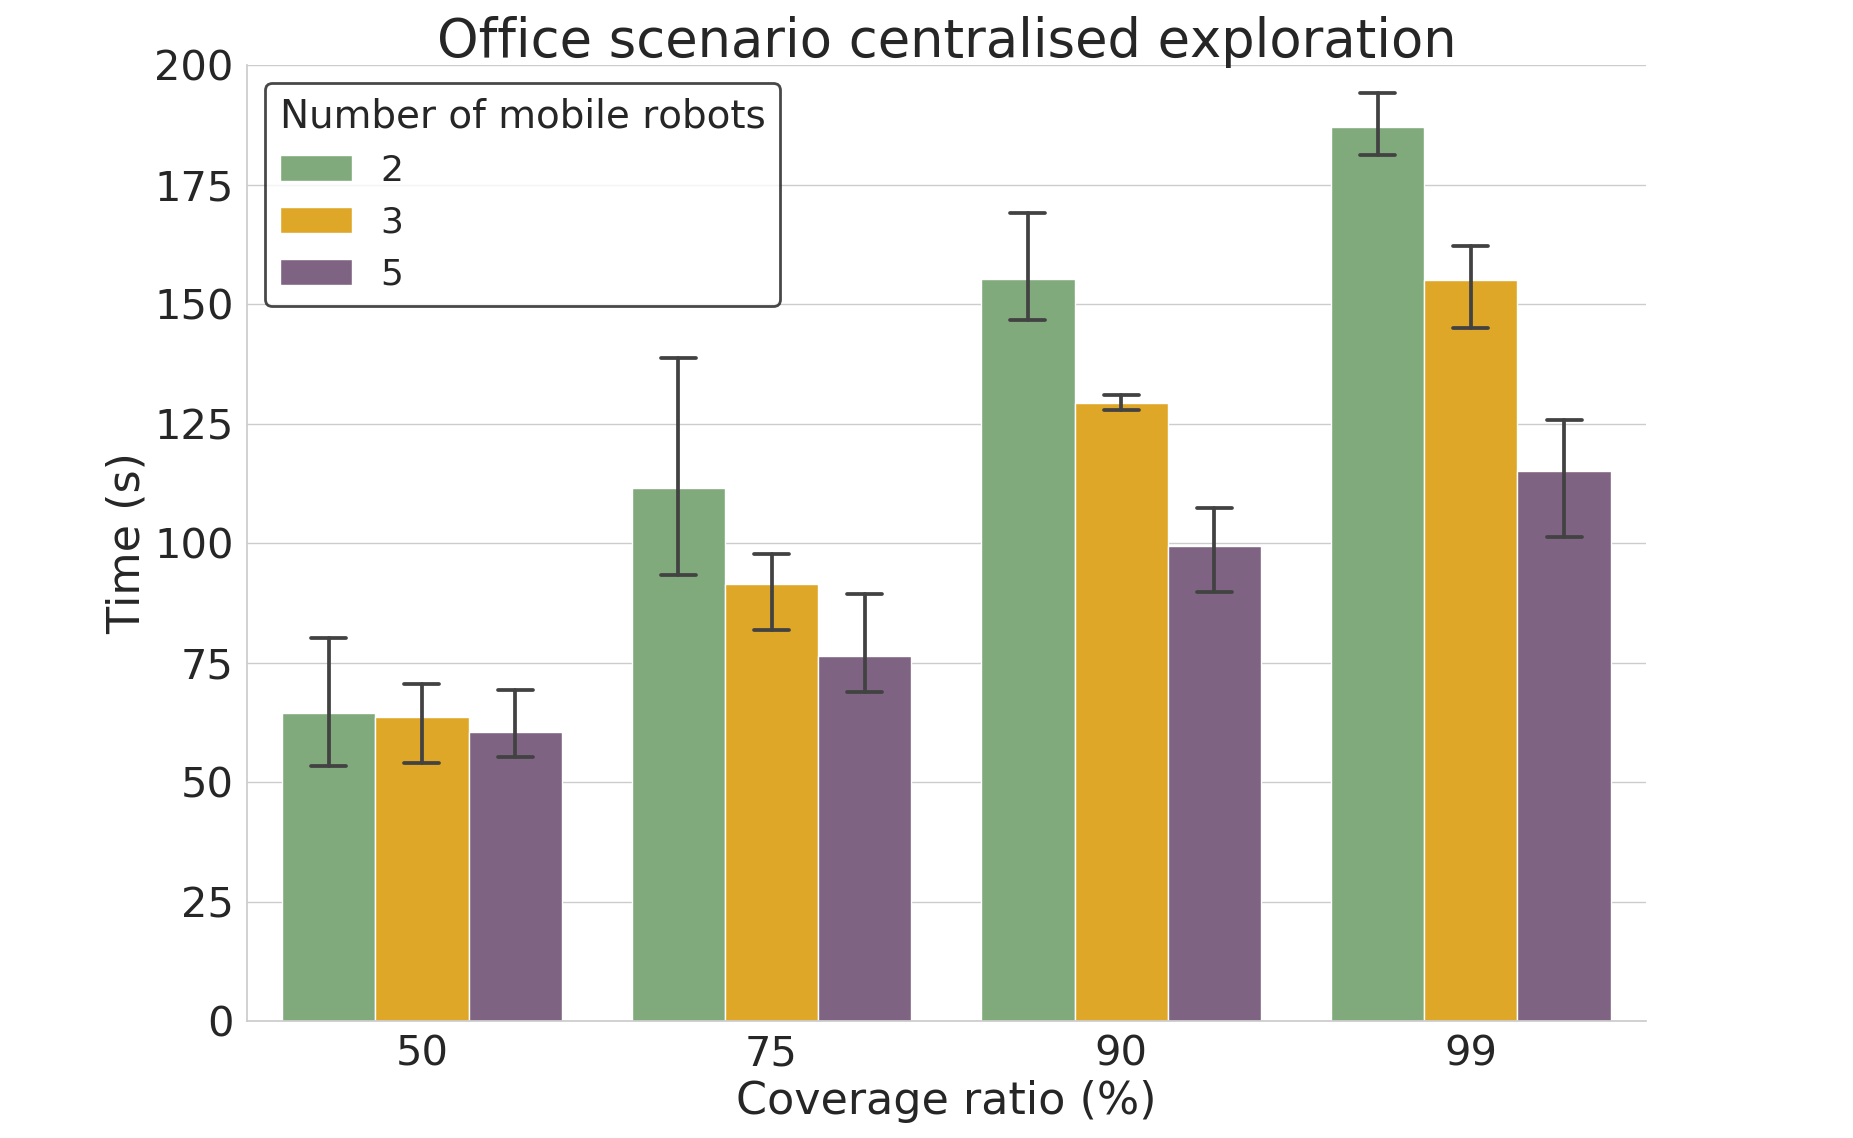
\includegraphics[width=0.46\textwidth]{office_c_cent.png}
        }\hfill
        \subfigure[\hspace{0.1cm} Coverage ratio over time in the office scenario for decentralised multi-robot exploration.]{%
           \label{fig:office_coverage_d}
           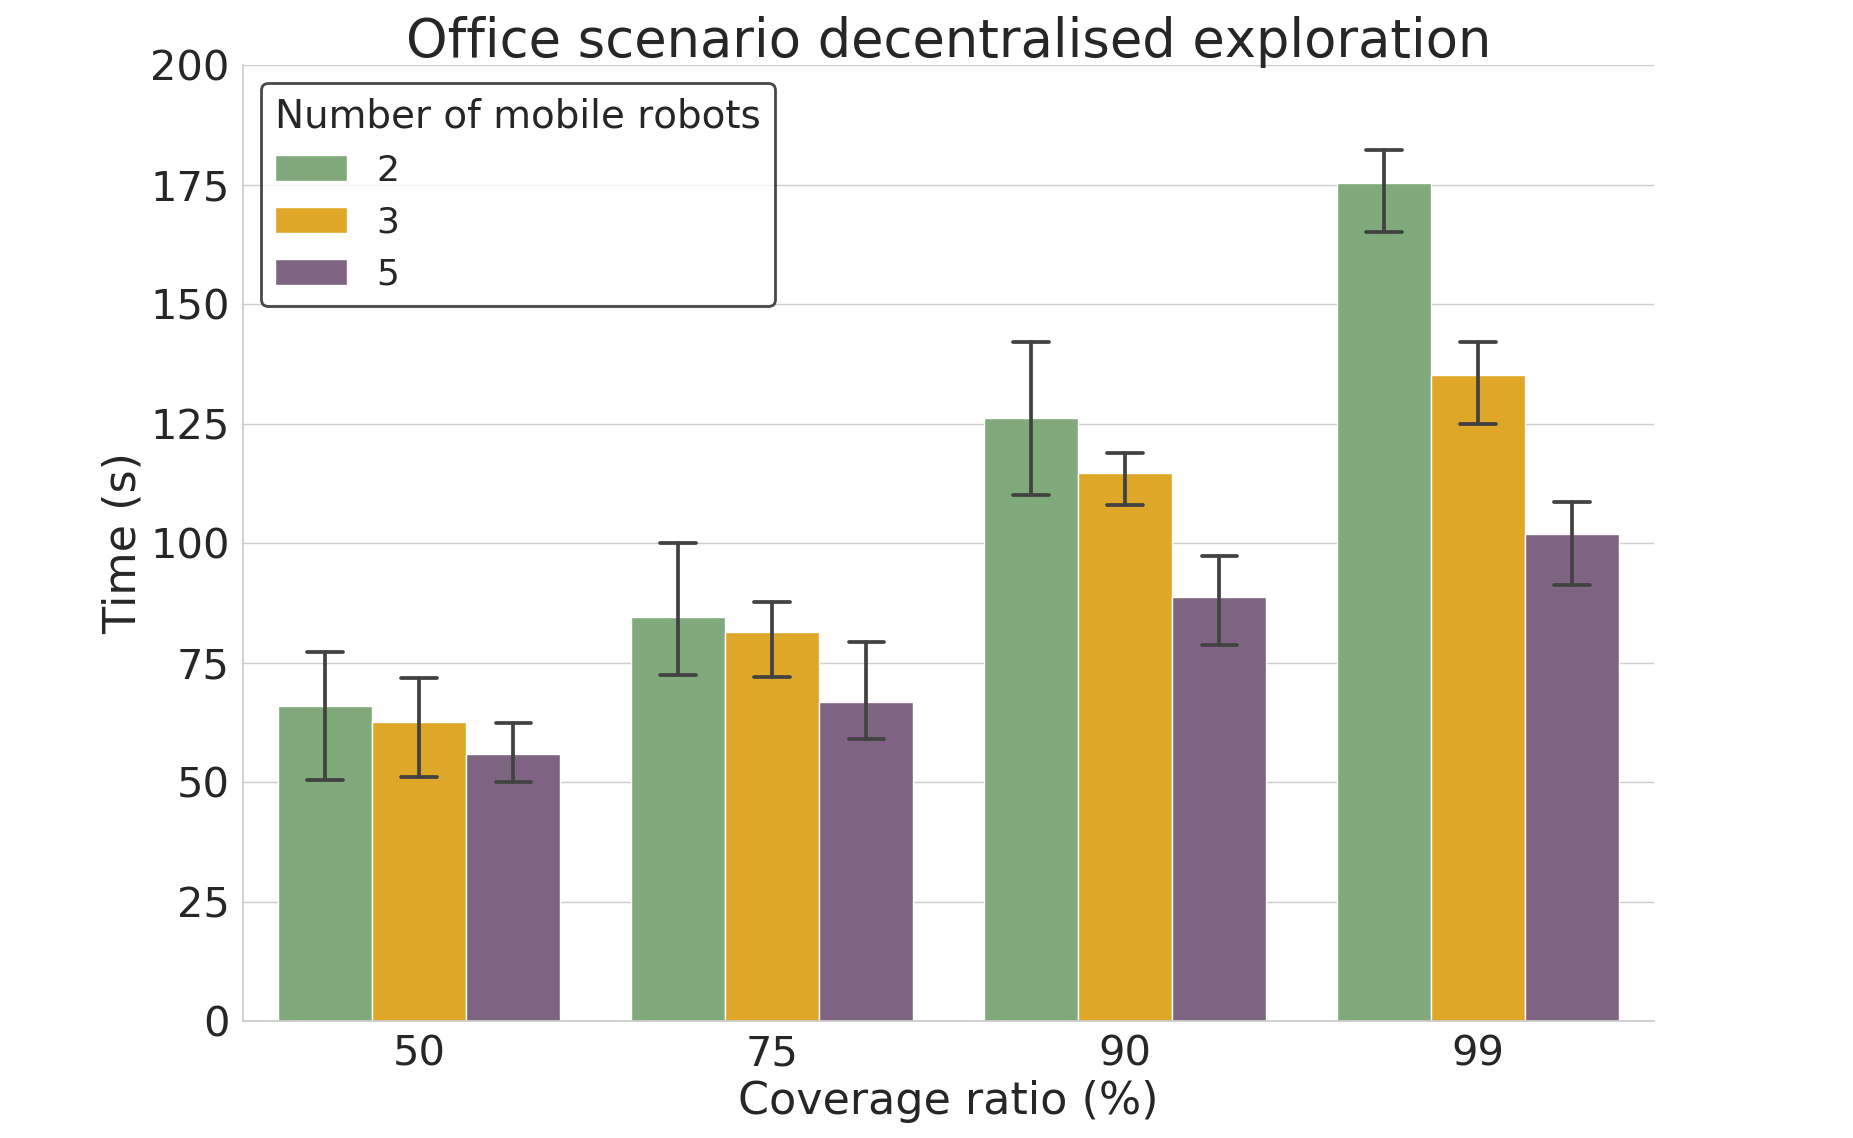
\includegraphics[width=0.46\textwidth]{office_c_decent.png}
        }\\ %  ------- End of the first row ----------------------%
        \subfigure[\hspace{0.1cm} Coverage ratio over time in the unstructured scenario for centralised multi-robot exploration.]{%
            \label{fig:unstruc_coverage_c}
            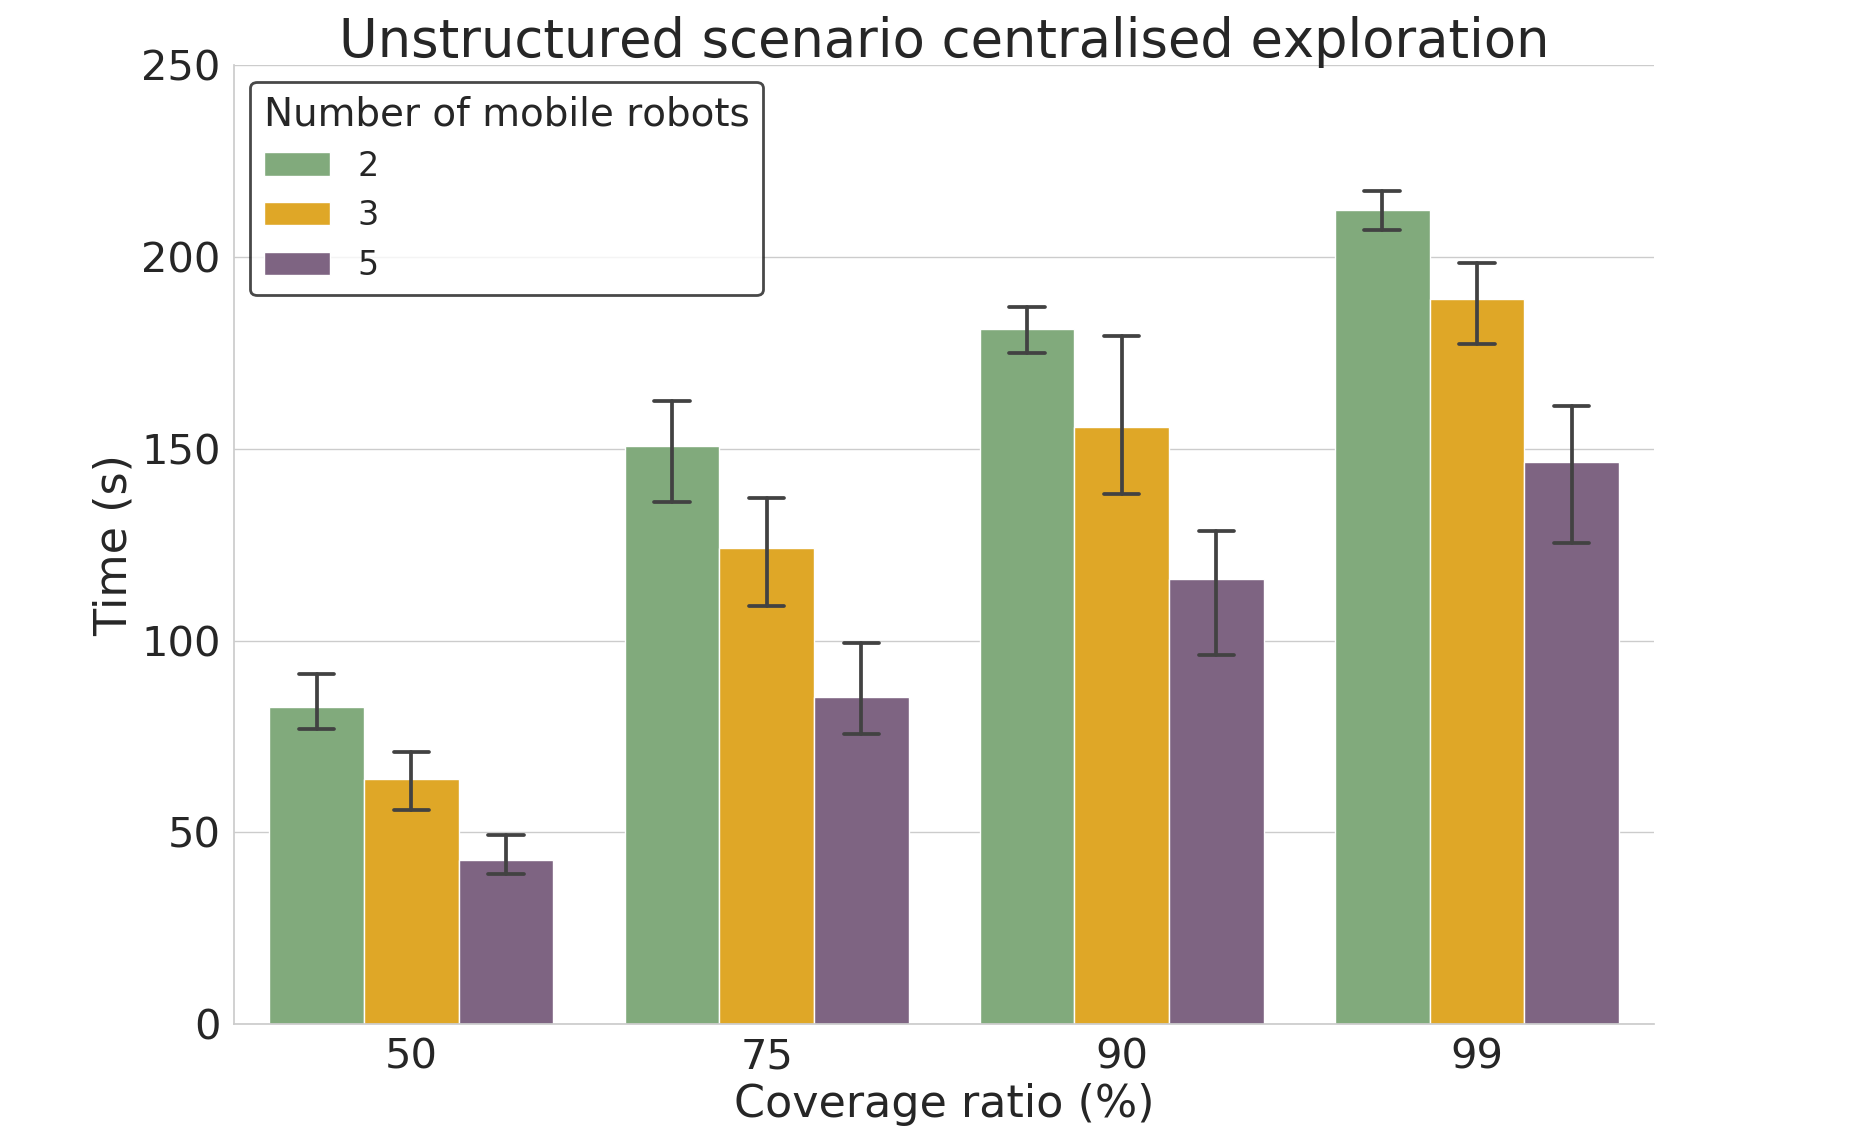
\includegraphics[width=0.46\textwidth]{unstructured_c_cent.png}
        }\hfill
        \subfigure[\hspace{0.1cm} Coverage ratio over time in the unstructured scenario for decentralised multi-robot exploration.]{%
            \label{fig:unstruc_coverage_d}
            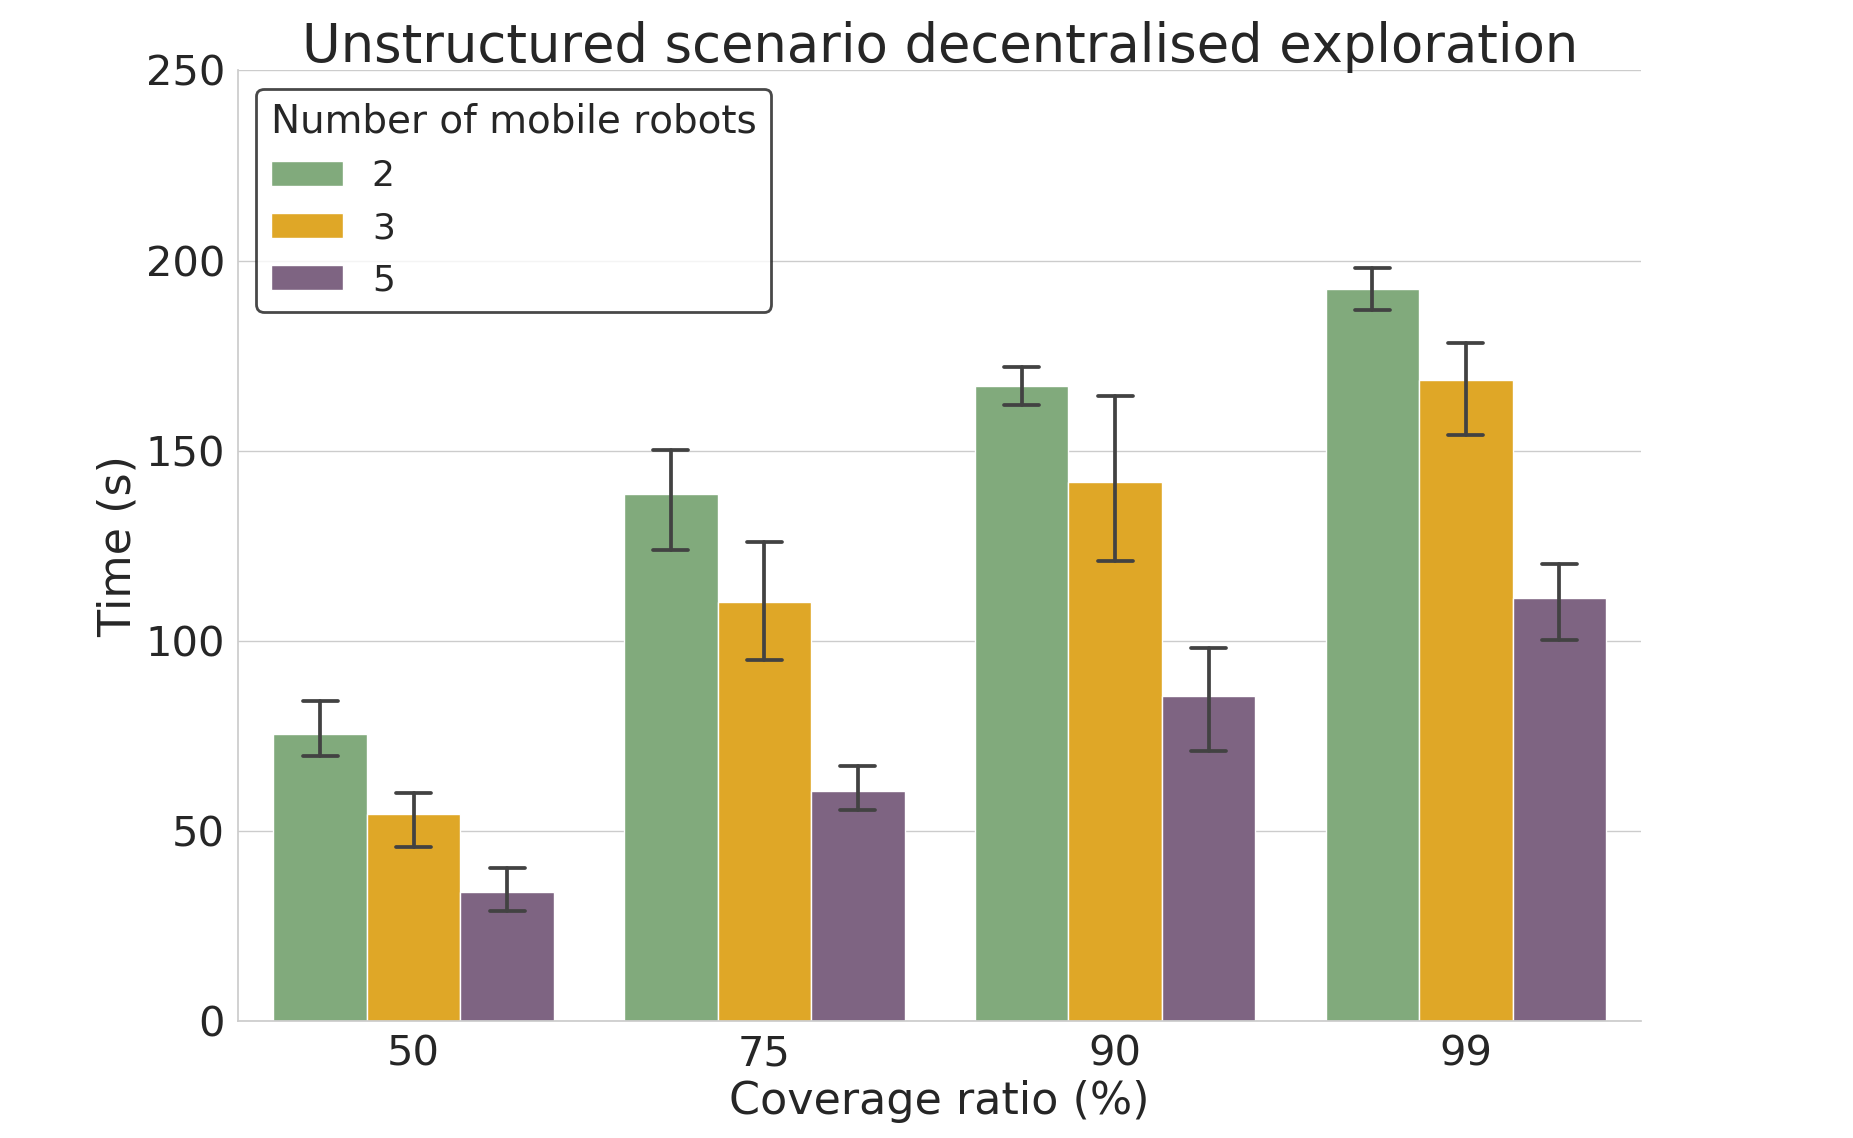
\includegraphics[width=0.46\textwidth]{unstructured_c_decent.png}
        }%
%
    \end{center}
    \caption{%
        The comparison of the coverage ratio over time during centralised and decentralised multi-robot exploration in the office scenario \subref{fig:office_coverage_c}, \subref{fig:office_coverage_d} and in the unstructured scenario \subref{fig:unstruc_coverage_c}, \subref{fig:unstruc_coverage_d}. 
     }%
   \label{fig:coverage_subfigures}
\end{figure*}

The frontier occupancy function $F_{ij}$ is the 2-dimensional Gaussian function with the position of the mean in a frontier point and with the standard deviation 
$3\sigma$= \begin{bmatrix}
           r_{f} \\
           r_{f} 
   \end{bmatrix}.
   
 If the frontier point $j$, for which the mobile robot $i$ is calculating the weight, is in the range of radius $r_{f}$ from the position of the mobile robot assigned point (\boldsymbol{q_{a}}); the value of the frontier occupancy function is calculated by Gaussian function, and zero otherwise (\ref{eq:frontier_funct}).

\begin{equation}\label{eq:frontier_funct}
 F_{ij}=
\begin{cases} 
       \lambda_{f} e^{-\Big[\frac{(q_{jx} - q_{ax})^2}{2\sigma_{x}^2} + \frac{(q_{jy} - q_{ay})^2}{2\sigma_{y}^2}\Big]} & \text{if $d(\boldsymbol{q_{j}}, \boldsymbol{q_{a}})< r_{f}$}, \\
      \quad \quad \quad \quad \quad 0 & \text{otherwise}
   \end{cases}
\end{equation}

where $\lambda_{f}$ is an experimentally determined constant. 

The function $F_{ij}$ is used to prevent assigning the frontier point to the mobile robot B if that point is close to a point already assigned to mobile robot A. The example of the frontier point $j$ and its radii $r$ and $r_{f}$ is shown in Fig. \ref{fig:radijusi}.

\begin{figure}[b!]
	\centering
	\fbox{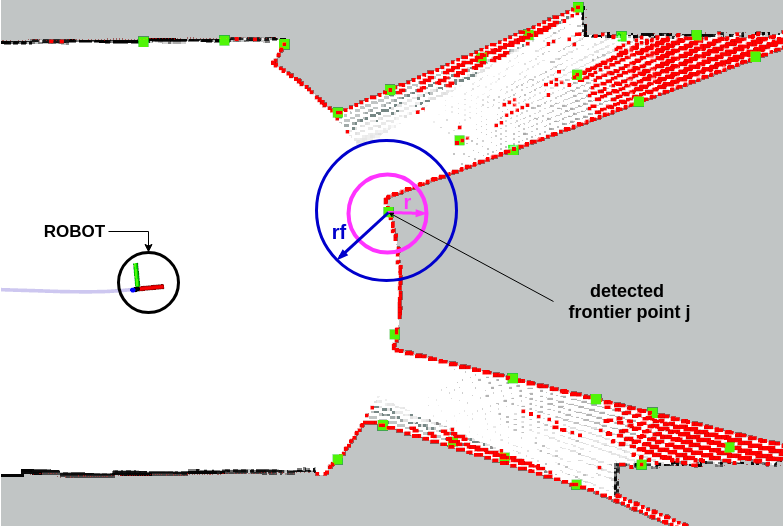
\includegraphics[width=0.85\columnwidth]{rviz_radius_vol4.png}}
	\caption{Detected frontier point $j$ and its radii $r$ and $r_{f}$.}
	\label{fig:radijusi}
\end{figure}

For each frontier point $j$, the weight $W_{ij}$ of the $i$-th mobile robot is calculated as: 
\begin{equation}
   {W}_{ij}= {C_{ij}} - {U_{ij}} + {F_{ij}}.
   \label{weight}
\end{equation}

The weight matrix $\boldsymbol{W}$ ($N\times M$) is formed for $N$ mobile robots and $M$ frontier points: 

\begin{equation}
    \boldsymbol{W} = \begin{bmatrix}
    W_{00} & W_{01} & \hdots & W_{0j} & \hdots & W_{0M}\\
    W_{10} & \ddots & & & & \vdots\\
    \vdots & & \ddots & & &  \vdots \\
    W_{i0} & & & \ddots & & \vdots \\
    \vdots & & & & \ddots & \vdots\\
    W_{N0} & \hdots  & \hdots  & \hdots  & \hdots &    W_{NM}
    \end{bmatrix}.
\end{equation}

The mobile robots exchange the information about weights for all frontier points and make decisions for the future actions based on the exchanged information. The amount of exchanged data is thus reduced, which allows for easier and faster communication.
The weight matrix $\boldsymbol{W}$ represents the input into the Hungarian algorithm that attempts to find an optimal assignment solution in polynomial time.

The Hungarian algorithm is described in \cite{hungarian} and tested in \cite{comparison}. Initially, the Hungarian algorithm assumes that the number of frontier points is the same as the number of mobile robots. Due to the fact that there are usually fewer mobile robots than frontier points, virtual mobile robots are added and then skipped during the process of assignment and exploration.

Let the matrix $X$ be the matrix of zeros and ones, where $X[i,j]=1$ iff the mobile robot $i$ is assigned to the frontier point $j$.
Than the optimal task assignment has weight:

\begin{equation}
     {\mathrm{min}}\ \sum_{i} \sum_{j} W_{ij}\ X_{ij},
\end{equation}

anticipating that minimisation of sum will ensure the dispersion of the mobile robots in the environment. 

\begin{algorithm}[H]
\caption{Decentralised strategy for mobile robot $i$}
\label{algorithm1}
\begin{algorithmic}[1]
\For{ each frontier point $j$}
\State\hspace{\algorithmicindent} $W_{ij}$ = $C_{ij}$ - $U_{ij}$ + $F_{ij}$
\State\hspace{\algorithmicindent} Send $W_{ij}$ to the other mobile robots.
\State \hspace{\algorithmicindent} Receive the weights from the others.
\State \hspace{\algorithmicindent} Calculate weight matrix $\boldsymbol{W}$.
\State \hspace{\algorithmicindent} Hungarian algorithm ($\boldsymbol{W}$).
\State{\textbf{return} Mobile robot $i$ is assigned to frontier point.}
\EndFor
\end{algorithmic}
\end{algorithm}

Our decentralised strategy executes during the robot motion and there are seven steps for each robot to be executed (Algorithm \ref{algorithm1}).  All frontier points are visible to every mobile robot.
When mobile robot $i$ is assigned to frontier point according to line 7 in Algorithm \ref{algorithm1}, the mobile robot starts to follow the planned path and navigate to the target frontier point. Moreover, at the moment when the mobile robot $i$ reaches the target point, a weight calculation request is sent to the other mobile robots, whose responses fill in the weight matrix $\boldsymbol{W}$ (which is an input to Hungarian algorithm). The described process executes until the whole environment is explored, in other words, until a complete  map of the environment is generated.


\section{SIMULATION RESULT}

The proposed strategy is implemented and tested using the Robot Operating System (ROS) framework. In order to prove the efficiency of our decentralised strategy, we compared it with the coordinated centralised market model described in \cite{burgard}. Experiments were performed in the two different indoor environments (Fig. \ref{fig:scenarios}) with two, three and five mobile robots. The start pose of the mobile robot was the same for each run. The results are presented as average of 10 runs for each set. The simulation setup is shown in the Table \ref{tab:table1}.


\begin{figure}[t]
    \setcounter{subfigure}{0}
     \begin{center}
        \subfigure[][]{\label{fig:office}
            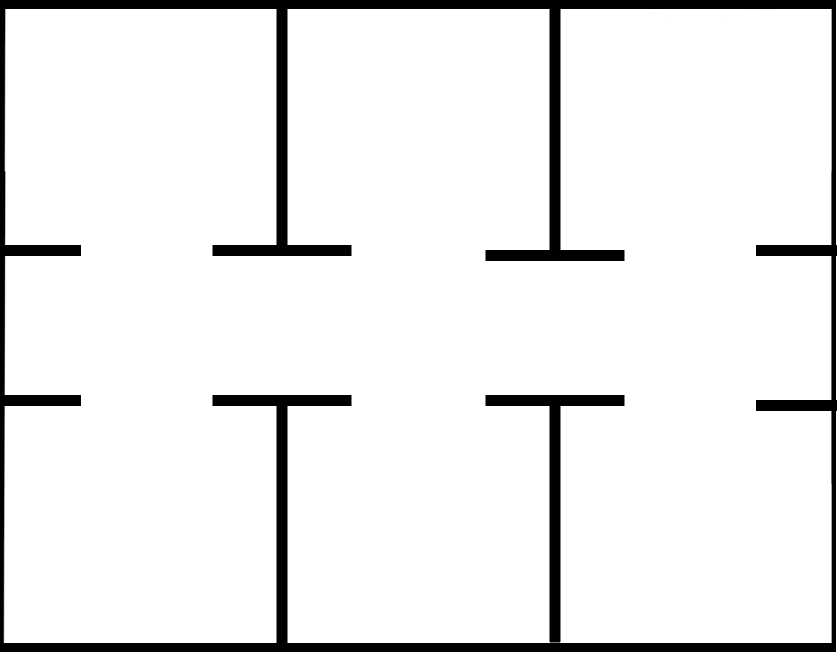
\includegraphics[width=0.47\columnwidth]{office1.png}
        }\hfill
        \subfigure[]{\label{fig:unstructured}
           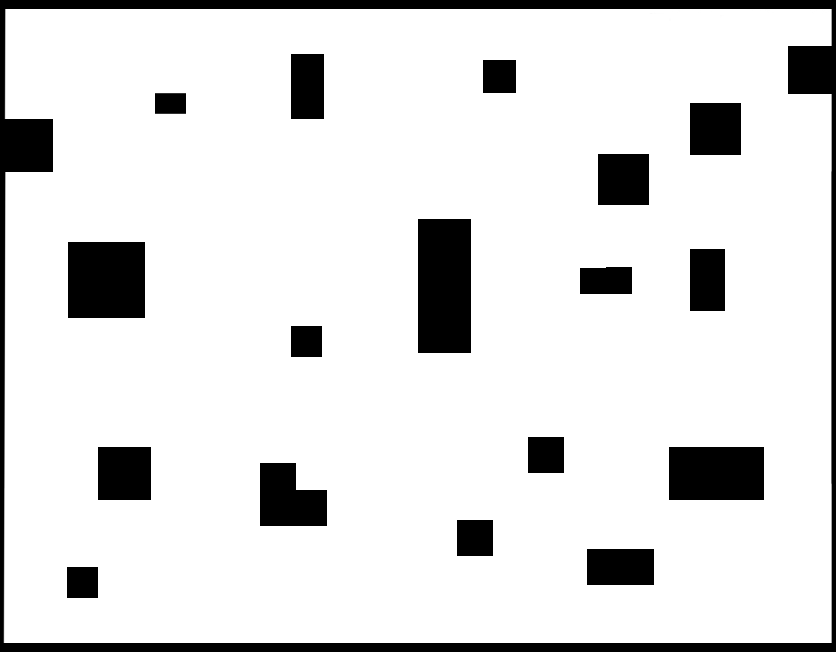
\includegraphics[width=0.47\columnwidth]{unstructured.png}}
    \end{center}
    \caption{%
       Benchmark scenarios. The terrains cover the flat surface 40 x 20 $m^{2}$ with static obstacles. \subref{fig:office} Office-like scenario; \subref{fig:unstructured} Unstructured scenario.
     }%
   \label{fig:scenarios}
\end{figure}




\begin{figure*}[h!]
     \begin{center}
     \setcounter{subfigure}{0}
%
        \subfigure[\hspace{0.1cm} Total exploration time for centralised and decentralised strategy in the office scenario for the different size of the mobile robot team]{%
            \label{fig:tt-office-a}
            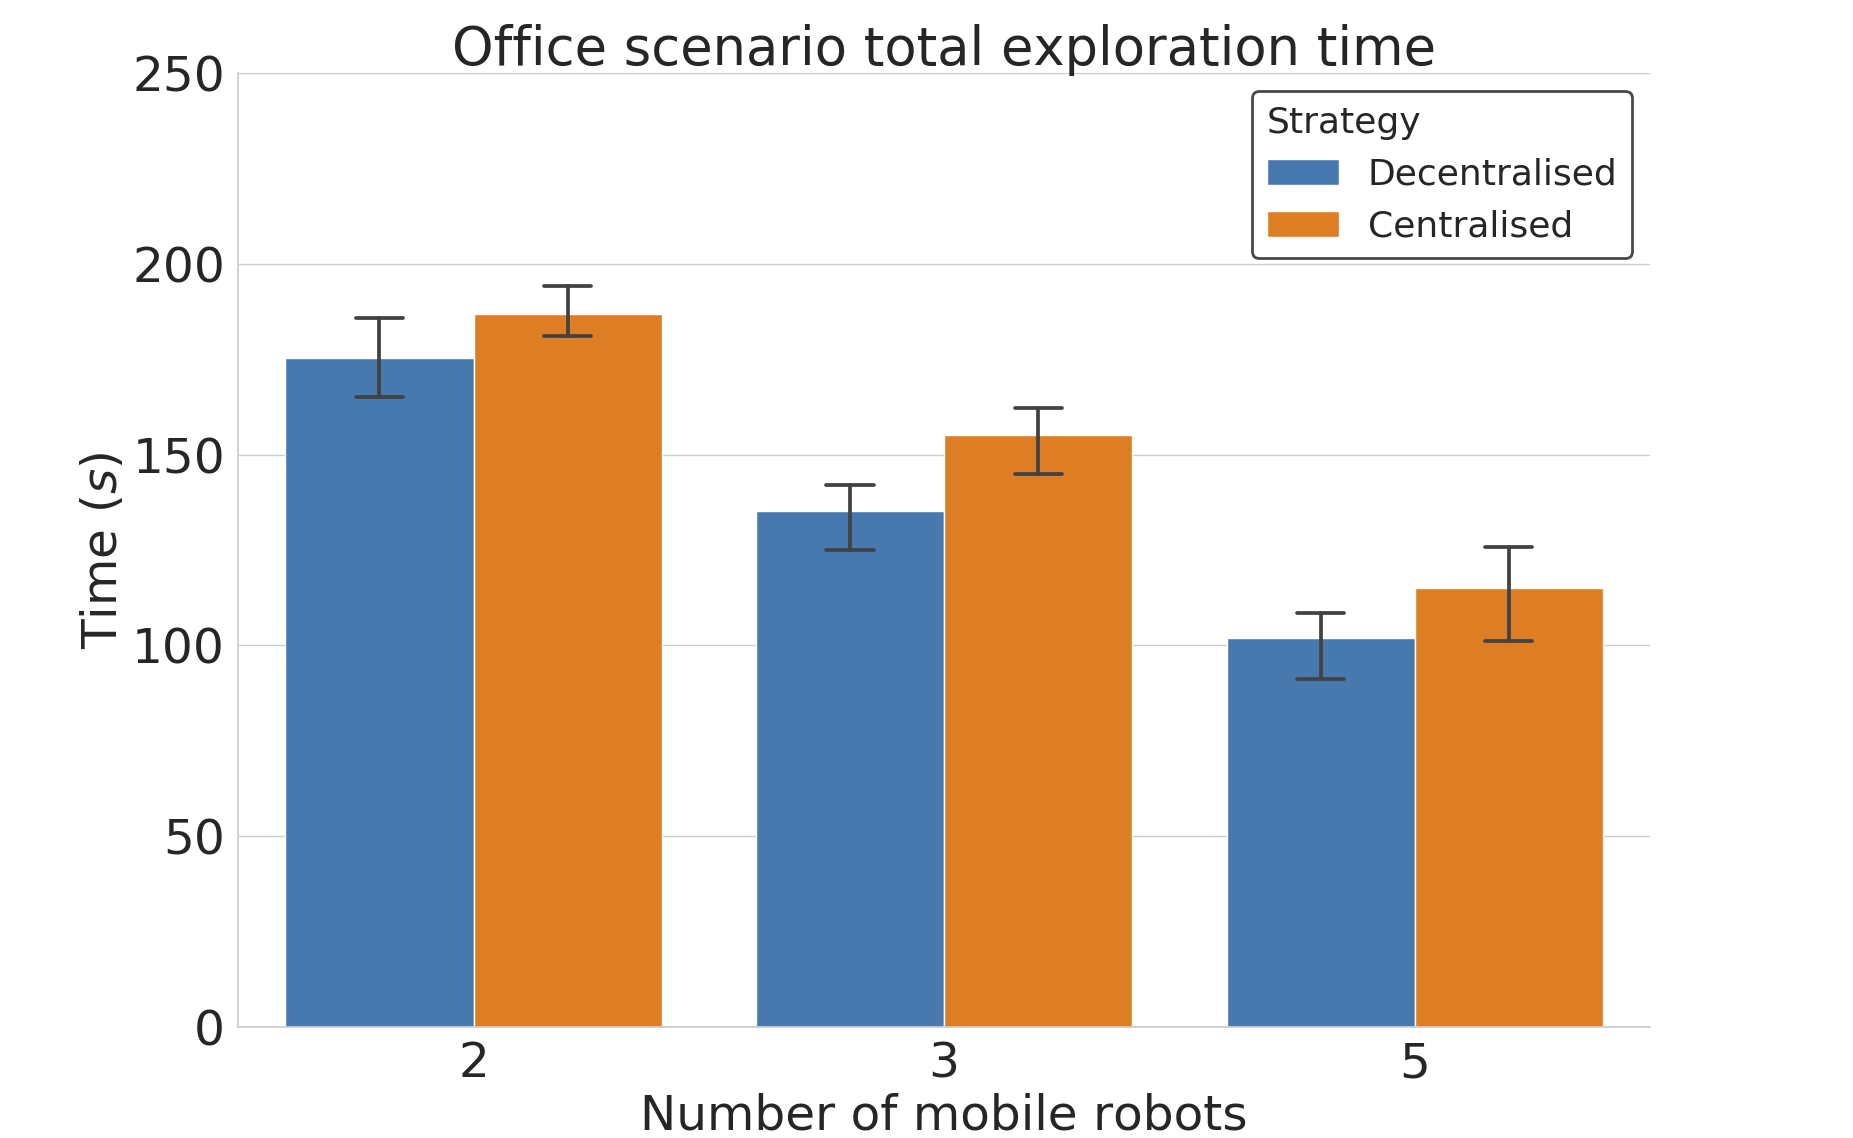
\includegraphics[width=0.46\textwidth]{office_total_e_time.png}
        }\hfill
        \subfigure[\hspace{0.1cm} Total exploration time for centralised and decentralised strategy in the unstructured scenario for the different size of the mobile robot team]{%
           \label{fig:tt-unstructired-b}
           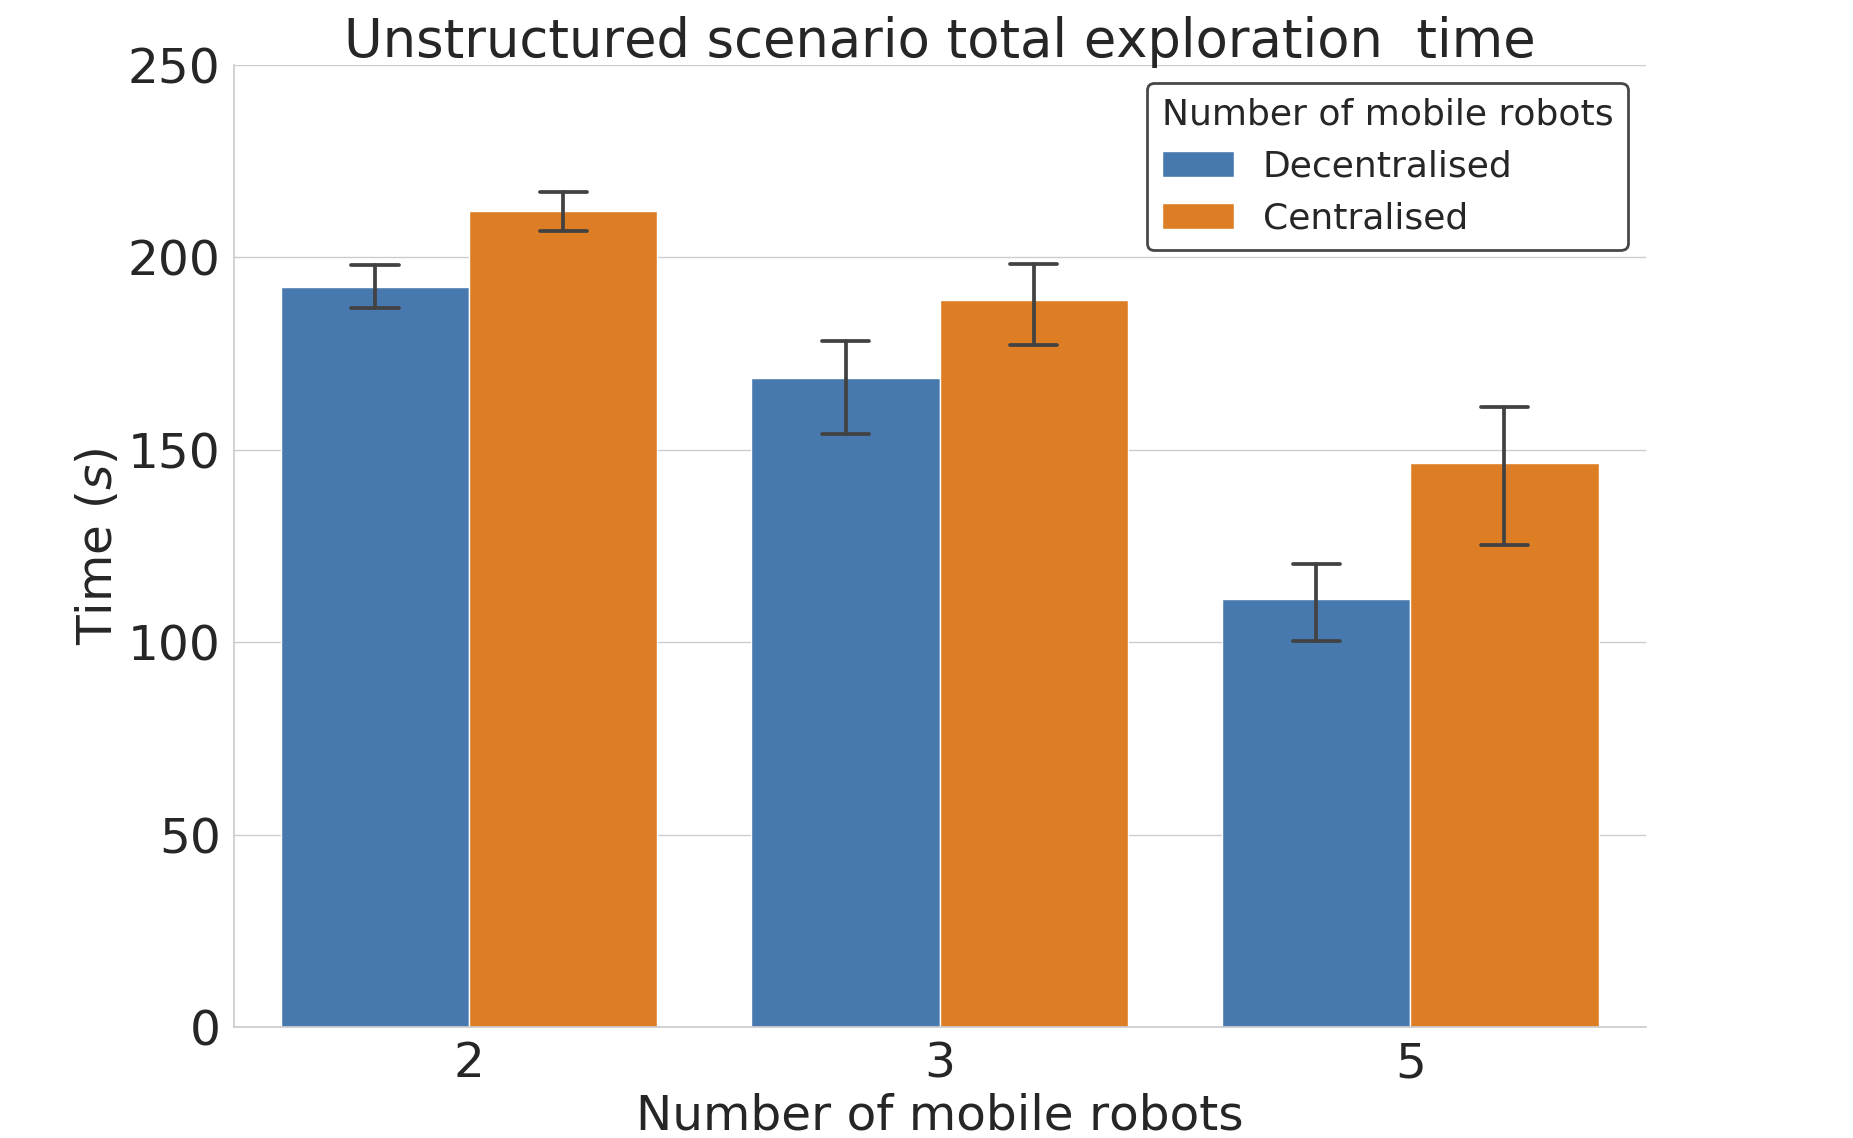
\includegraphics[width=0.46\textwidth]{unstructured_total_e_time.png}
        }\\ %  ------- End of the first row ----------------------%
        \subfigure[\hspace{0.1cm} Average path length per robot for centralised and decentralised strategy in the office scenario for the different size of the mobile robot team]{%
            \label{fig:path-office-c}
            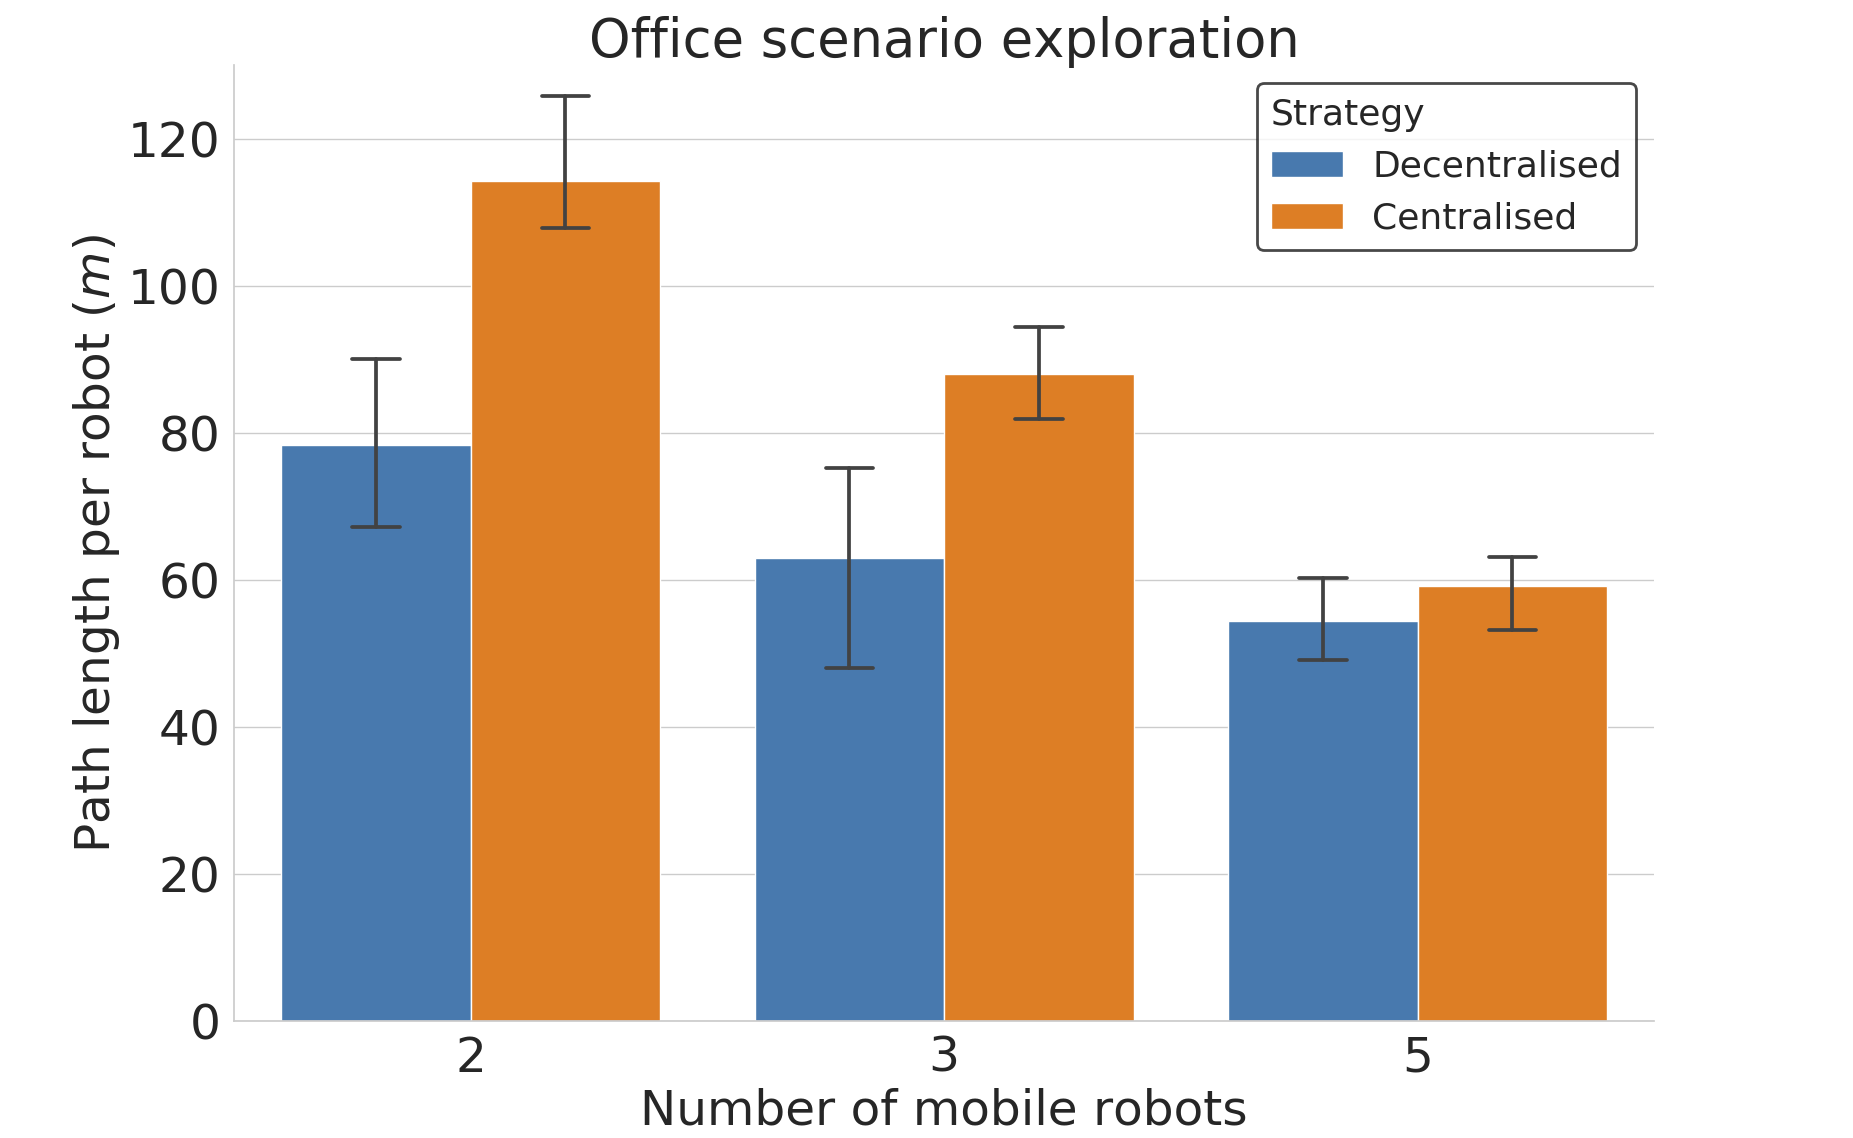
\includegraphics[width=0.46\textwidth]{office_path_length_per_robot.png}
        }\hfill
        \subfigure[\hspace{0.1cm} Average path length per robot for centralised and decentralised strategy in the unstructured scenario for the different size of the mobile robot team]{%
            \label{fig:path-unstructured-d}
            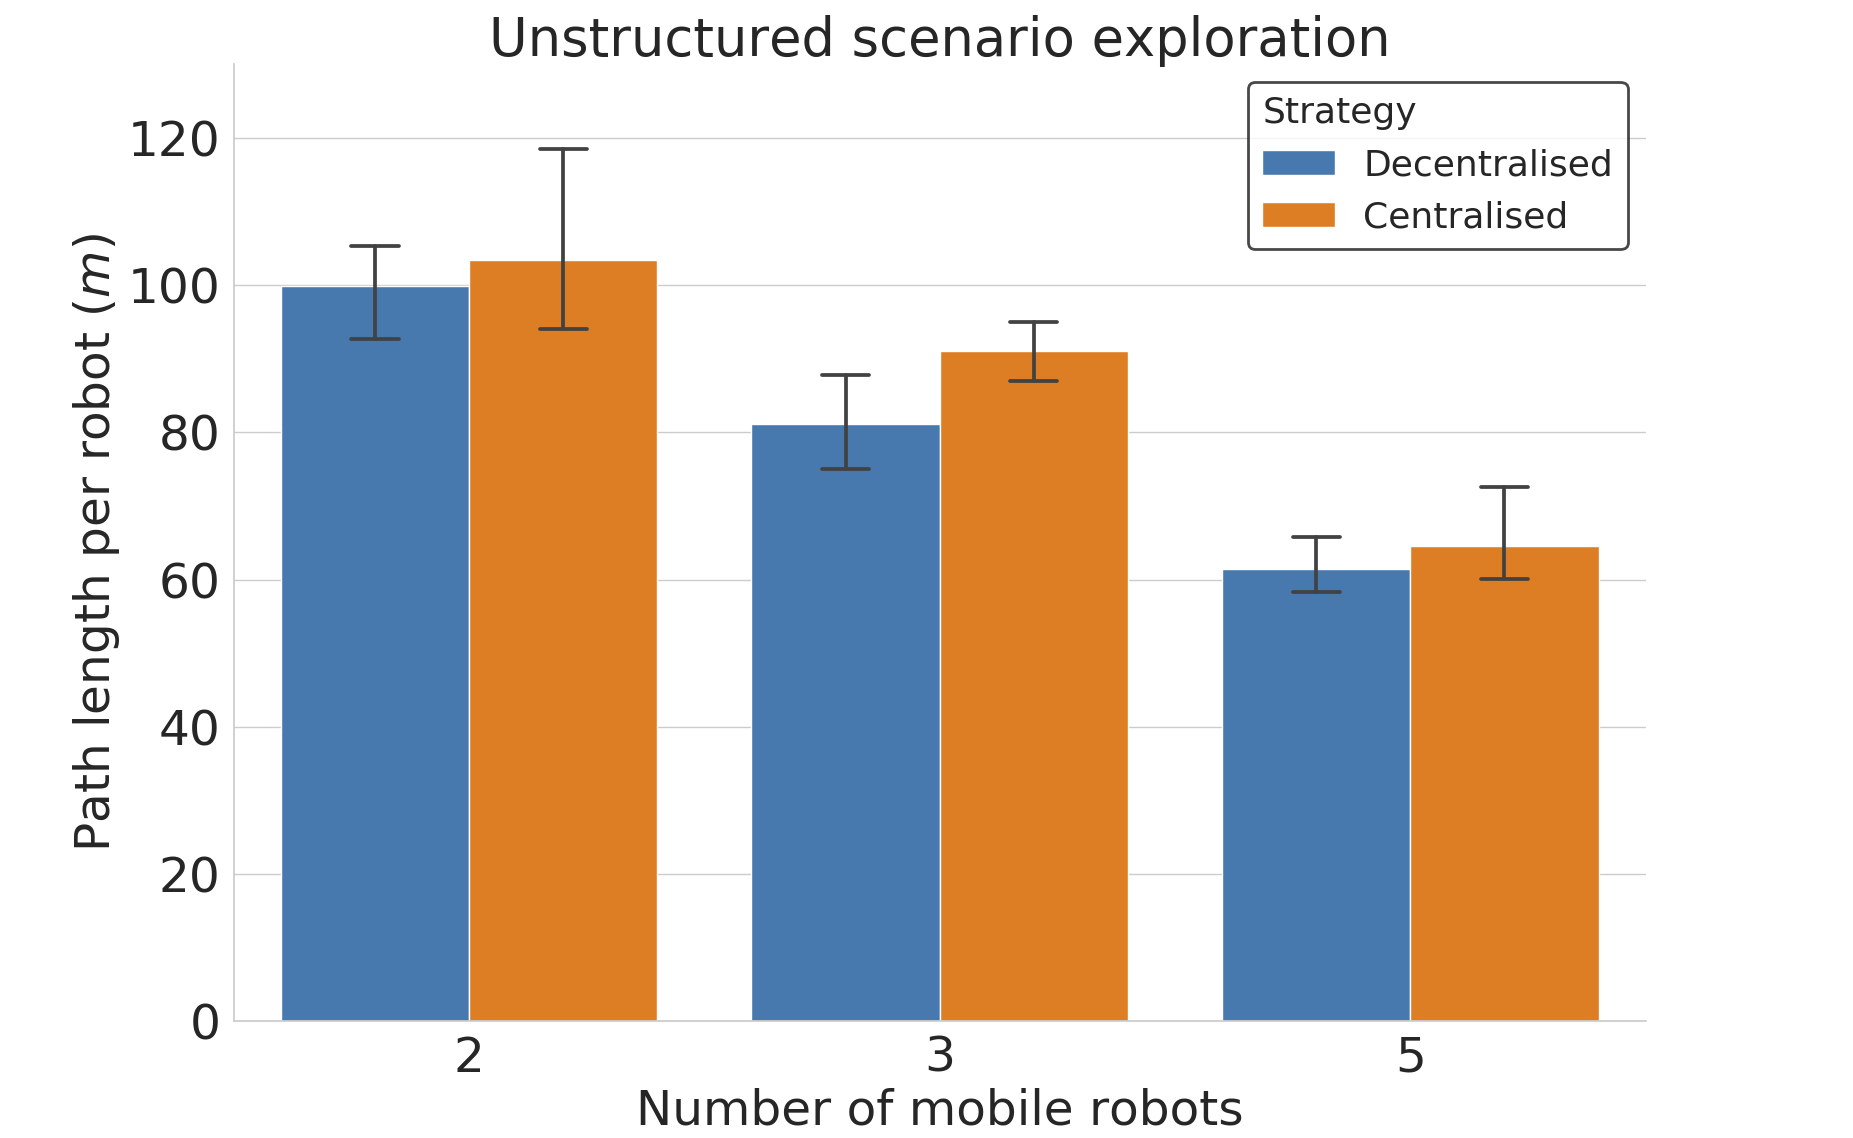
\includegraphics[width=0.46\textwidth]{unstructured_path_lenght_per_robot.png}
        }%
%
    \end{center}
    \caption{%
       The comparison of the centralised and decentralised strategy for office and unstructured scenarios in the term of total exploration time \subref{fig:tt-office-a}, \subref{fig:tt-unstructired-b} and in the term of path length per robot \subref{fig:path-office-c}, \subref{fig:path-unstructured-d}.
     }%
   \label{fig:time_and_path_subfigures}
\end{figure*}

\begin{table}[t]
  \centering
    \caption{Simulation setup.}
    \label{tab:table1}
    \begin{tabular}{ll} 
\hline
\rule{0pt}{2.2ex}
\textbf{Mobile robot features} &  \\ 
\quad Model & Pioneer P3-DX  \\
\quad Maximum speed & 1.5 (m/s) \\
\quad Laser range & 10 (m) \\
\quad Laser scan window & 250 ($^{\circ}$) \\
\hline
\rule{0pt}{2.2ex}
\textbf{Environment features}  \\ 
\quad Terrain & 40 x 20 ({m}^2) \\
\quad Wall height & 0.5 (m) \\
\quad Initial mobile robot position & Center \\
\hline
\rule{0pt}{2.2ex}
\textbf{Decentralised strategy parameters} & \\
\quad  \lambda_{u} & 0.9\\
\quad \lambda_{f} & 1.2\\
\quad $r$ & 1.0\\
\quad $r_{f}$ & 3.0\\
\hline
\rule{0pt}{2.2ex}
%\quad Intel Core i7-8550U @ 1.80GHz & \\
\end{tabular}
\end{table}

The comparison of the centralised strategy and our decentralised strategy is shown in Fig. \ref{fig:coverage_subfigures} and Fig. \ref{fig:time_and_path_subfigures} using the indicators defined as follows:

\textbf{Coverage Ratio (CR)}: percentage of the accessible terrain covered by the team. Calculated as:  \( \frac{\text{explored cells} \cdot 100}{\text{accessible cells}} \).

\textbf{Path Length (PL)}: distance travelled by a mobile robot measured in meters.

\textbf{Total exploration Time (TT)}: time elapsed from the beginning until the end of exploration measured in seconds.\\

First of all, it is interesting to see how the coverage evolves over time. Fig. \ref{fig:coverage_subfigures} shows \textbf{CR} over time for both centralised and decentralised multi-robot exploration strategies in the office scenario as well as in the unstructured scenario. We report the time it takes to cover 50, 75, 90 and 99 percent of the environment. Obviously, it takes almost the same time to explore a few last cells and 25 percent (from 75 to 90 percent) of the environment. In the both scenarios, the decentralised strategy needed less time to explore the same percentage of the environment. Furthermore, increase in performance was greater for larger number of mobile robots. For instance, using decentralised strategy, it took 14 percent less time for three mobile robots to explore unstructured environment compared to centralised strategy, and for five mobile robots the increase was 25 percent.  

When we compare the \textbf{TT} for the both strategies (Fig. \ref{fig:time_and_path_subfigures} \subref{fig:tt-office-a} and \subref{fig:tt-unstructired-b}), it shows that five mobile robots perform better than two and three, while there is a small difference in having three robots instead of two. The decentralised strategy performs faster than the centralised strategy.

The next parameter of interest for comparison is \textbf{PL} shown in the Fig. \ref{fig:time_and_path_subfigures} \subref{fig:path-office-c} and \subref{fig:path-unstructured-d}. We compared the average path length per robot for the different sizes of the mobile robot team for both strategies. The average path length per robot in the centralised strategy based on \cite{burgard} is significantly higher compared to the proposed decentralised strategy, especially in the office scenario for two and three mobile robots. 



\section{CONCLUSION AND FUTURE WORK}
We have presented an approach to autonomous decentralised multi-robot exploration and mapping based on the market model. This strategy has demonstrated improved behaviour compared to the centralised strategy that explicitly coordinates the robots, based on estimates of expected information gain and the cost of exploration. This includes both reduced total exploration time and path length per robot.

However, the approach described in this paper is limited in two aspects. First, in this work the filter module reduces the number of the frontier points by removing the points that are too close to each other. We are investigating improved frontier point filtering and clustering, which we believe will improve overall performance significantly. And second, all mobile robots communicate to each other and create a fully connected graph. If the communication range is limited and it is assumed that just the mobile robots close to each other can communicate and negotiate, coordinated exploration can still be performed, trading off quality of coordination for smaller required communication bandwidth.

\addtolength{\textheight}{-12cm}   % This command serves to balance the column lengths
                                  % on the last page of the document manually. It shortens
                                  % the textheight of the last page by a suitable amount.
                                  % This command does not take effect until the next page
                                  % so it should come on the page before the last. Make
                                  % sure that you do not shorten the textheight too much.

%%%%%%%%%%%%%%%%%%%%%%%%%%%%%%%%%%%%%%%%%%%%%%%%%%%%%%%%%%%%%%%%%%%%%%%%%%%%%%%%

\begin{thebibliography}{99}

\bibitem{free-market} B. Dias, S. Stentz, A free market architecture for distributed control of a multirobot system, in 6th International Conference on Intelligent Autonomous Systems, pp. 115-122, 2000.

\bibitem{burgard} W. Burgard, M. Moors, C. Stachniss, and F. Schneider. Coordinated multi-robot exploration. IEEE Transactions on Robotics, 21(3):376–378, 2005.

\bibitem{hungarian} H.W. Kuhn, The Hungarian method for the assignment problem, Naval Research Logistics Quarterly, 2(1):83–97, 1955.

\bibitem{planetary} M.J. Matarić and G. Sukhatme, Task-allocation and coordination of multiple robots for planetary exploration, in Proc. of the Int. Conf. on Advanced Robotics (ICAR), pages 61–70, Budapest, Hungary, 2001.

\bibitem{Yamauchi} B. Yamauchi, Frontier-based exploration using multiple robots, in Proc. of the Second International Conference on Autonomous Agents, pages 47–53, Minneapolis, MN, USA, 1998.

\bibitem{market-economy} R. Zlot, A.T. Stenz, M.B. Dias, and S. Thayer, Multi-robot exploration controlled by a market economy, in Proc. of the IEEE Int. Conf. on Robotics and Automation (ICRA), Washington, DC, USA, 2002.

\bibitem{rescue} R. Murphy, Human-robot interaction in rescue robotics, IEEE Syst., Man, Cybern., C, Appl. Rev., vol. 34, no. 2, pp. 138–153, May 2004.

\bibitem{cleaning1} H. Endres, W. Feiten, and G. Lawitzky, Field test of a navigation system: autonomous cleaning in supermarkets, in Proc. IEEE Int. Conf. Robot. Autom. (ICRA), pp. 1779–1781, 1998.

\bibitem{cleaning2} P. Pinheiro, E. Cardozo, J. Wainer, and E. RohmerCleaning, Task planning for an autonomous robot in indoor places with multiples rooms, International Journal of Machine Learning and Computing, Vol. 5, No. 2, April 2015.

\bibitem{segmentation} K. M. Wurm, C. Stachniss, and W. Burgard, Coordinated multi-robot exploration using a segmentation of the environment, in Proc. IEEE/RSJ  International Conference on Intelligent Robots and Systems (IROS), September 2008.

\bibitem{Julia} M. Julia, A. Gil, and O. Reinoso, A comparison of path planning strategies for autonomous exploration and mapping of unknown environments, Autonomous Robots, vol. 33, no. 4, pp. 427–444, 2012. 

\bibitem{comparison} M. Kulich, T. Juchelka, and L. Preucil, Comparison of exploration strategies for multi-robot search, Acta Polytech, 55(3):162, June 2015. 

\bibitem{survey-analysis} M. B. Dias, R. Zlot, N. Kalra, and A. Stentz, Market-based multirobot coordination: A survey and analysis, Proc. of the IEEE 94 (7), 1257-1270, 2006.

\bibitem{Umari} H.Umari, and S. Mukhopadhyay, Autonomous robotic exploration based on multiple rapidly-exploring randomized trees,  in Proc. IEEE/RSJ International Conference on Intelligent Robots and Systems (IROS), Vancouver, BC, Canada, September 2017.

\bibitem{usporedba} M. B. Dias, and A. Stentz, A comparative study between centralized, market-based, and behavioral multirobot coordination approaches, in Proc. of the 2003 IEEE/RSJ  International Conference on In Intelligent Robots and Systems (IROS), Las Vegas, Nevada, October 2003.

\bibitem{Wurman} P. R. Wurman, R. D'Andrea, and M. Mountz, Coordinating hundreds of cooperative, autonomous vehicles in warehouses, in Proc. IAAI'07 Proceedings of the 19th national conference on Innovative applications of artificial intelligence, vol. 2, pp. 1752-1759, Vancouver, British Columbia, Canada, July 2007
 
\bibitem{behavioural} H. Lau, Behavioural approach for multi-robot exploration, Proc. of 2003 Australasian Conference on Robotics and Automation, Brisbane, Australia, December 2003

\bibitem{cartographer} W.  Hess,  D.  Kohler,  H.  Rapp,  and  D.  Andor, Real-time  loop  closure in  2d  lidar  slam, in Robotics  and  Automation  (ICRA), 2016  IEEE International Conference on. IEEE, 2016, pp. 1271–1278

\bibitem{juraj} J. Orsulic, D. Mikic and Z. Kovacic, Efficient dense frontier detection for 2D GraphSLAM based on occupancy grid submaps, CoRR, abs/1902.11061, 2019

\bibitem{Stage} W. Woodall, http://wiki.ros.org/stage

\bibitem{Yan} Z. Yan, N. Jouandeau and A. A. Cherif, A survey and analysis of multi-robot coordination, International Journal of Advanced Robotic Systems, Epub ahead of print 1 January 2013

\bibitem{Michael} N. Michael, M. M. Zavlanos, V. Kumar, and G. J. Pappas, Distributed multi-robot task assignment and formation control, in Proc. of ICRA'08, pages 128-133, Pasadena, CA, USA, May 2008.

\end{thebibliography}

\end{document}
